\documentclass[12pt]{article}
\usepackage{graphicx}
\graphicspath{ {./plots/} }
\usepackage{mathtools}
\usepackage{derivative}

\title{Deep learning in C}
\author{Jia Geng Chang }
\date{December 2021}


\begin{document}

\section{Self-supervised learning}

\subsection{Encoding a 8-bit one-hot vector with 3 bits}

I trained a multi-layer perceptron to encode with 3 units a one-hot encoded vector of length 8  e.g. \begin{pmatrix}0 & 0 & 0 & 0 & 0 & 0 & 1 & 0\end{pmatrix} which represents the value 7. Because only one value can be 1, there are only 8 such vectors — a relatively easy pattern for the network to learn to encode and decode.

With standard gradient descent, training was incredibly slow, even at high learning rates of up to 10. Thus, I added a momentum term involving the previous time step as a modification to vanilla gradient descent. The weight update heuristic at epoch $t$ becomes:
\begin{equation}
    \Delta W_{ij}(t) = -\eta \, \pdv{E}{W_{ij}} + m \,\Delta W_{ij}(t-1)
\end{equation}
for a pair of connected neurons $i$ and $j$, and m is scalar that practitioners suggest to be kept between 0 and 1. The result in training with varying $m$, for two different learning rates (lr = 0.01 and lr = 0.05) is shown below in figure \ref{fig:mlp_momentum}. 

\begin{figure}[htbp]
    \centering
    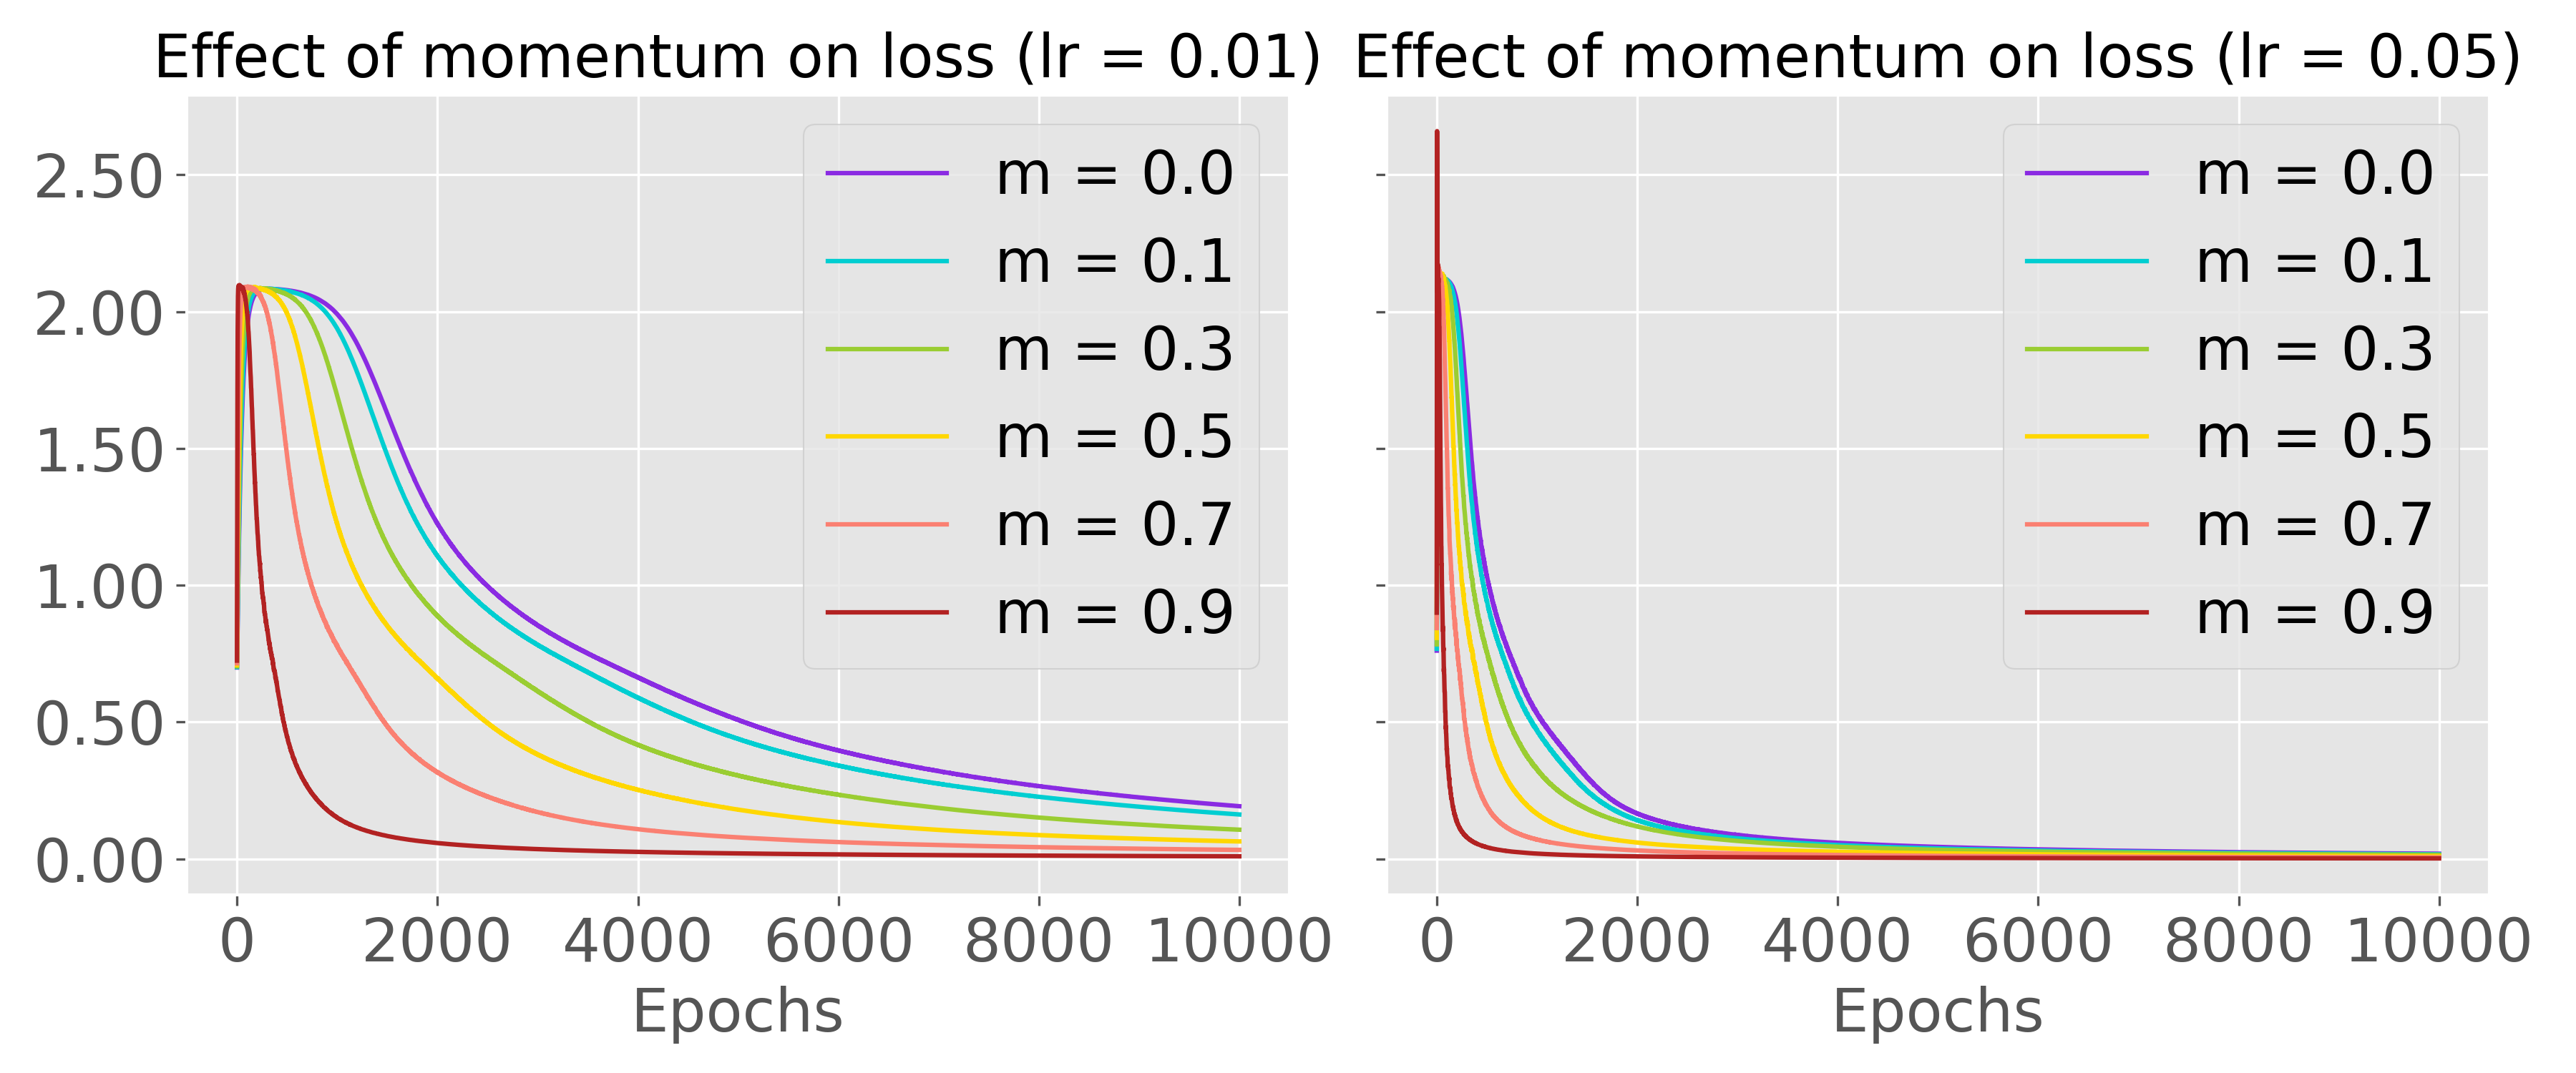
\includegraphics[width=12cm, height=5cm]{mlp_m}
    \caption{With learning rate held constant, momentum speeds up learning}
    \label{fig:mlp_momentum}
\end{figure}

We can see that adding momentum speeds up training greatly. What is happening is that the magnitude of $\Delta W_{ij}(t)$ is increasing by a factor of close to $1+m$ as a function of $t$.

How is the network learning to encode input vectors? We look at the final state of the weights for the best network to see what is happening.

\begin{figure}[htbp]
    \centering
    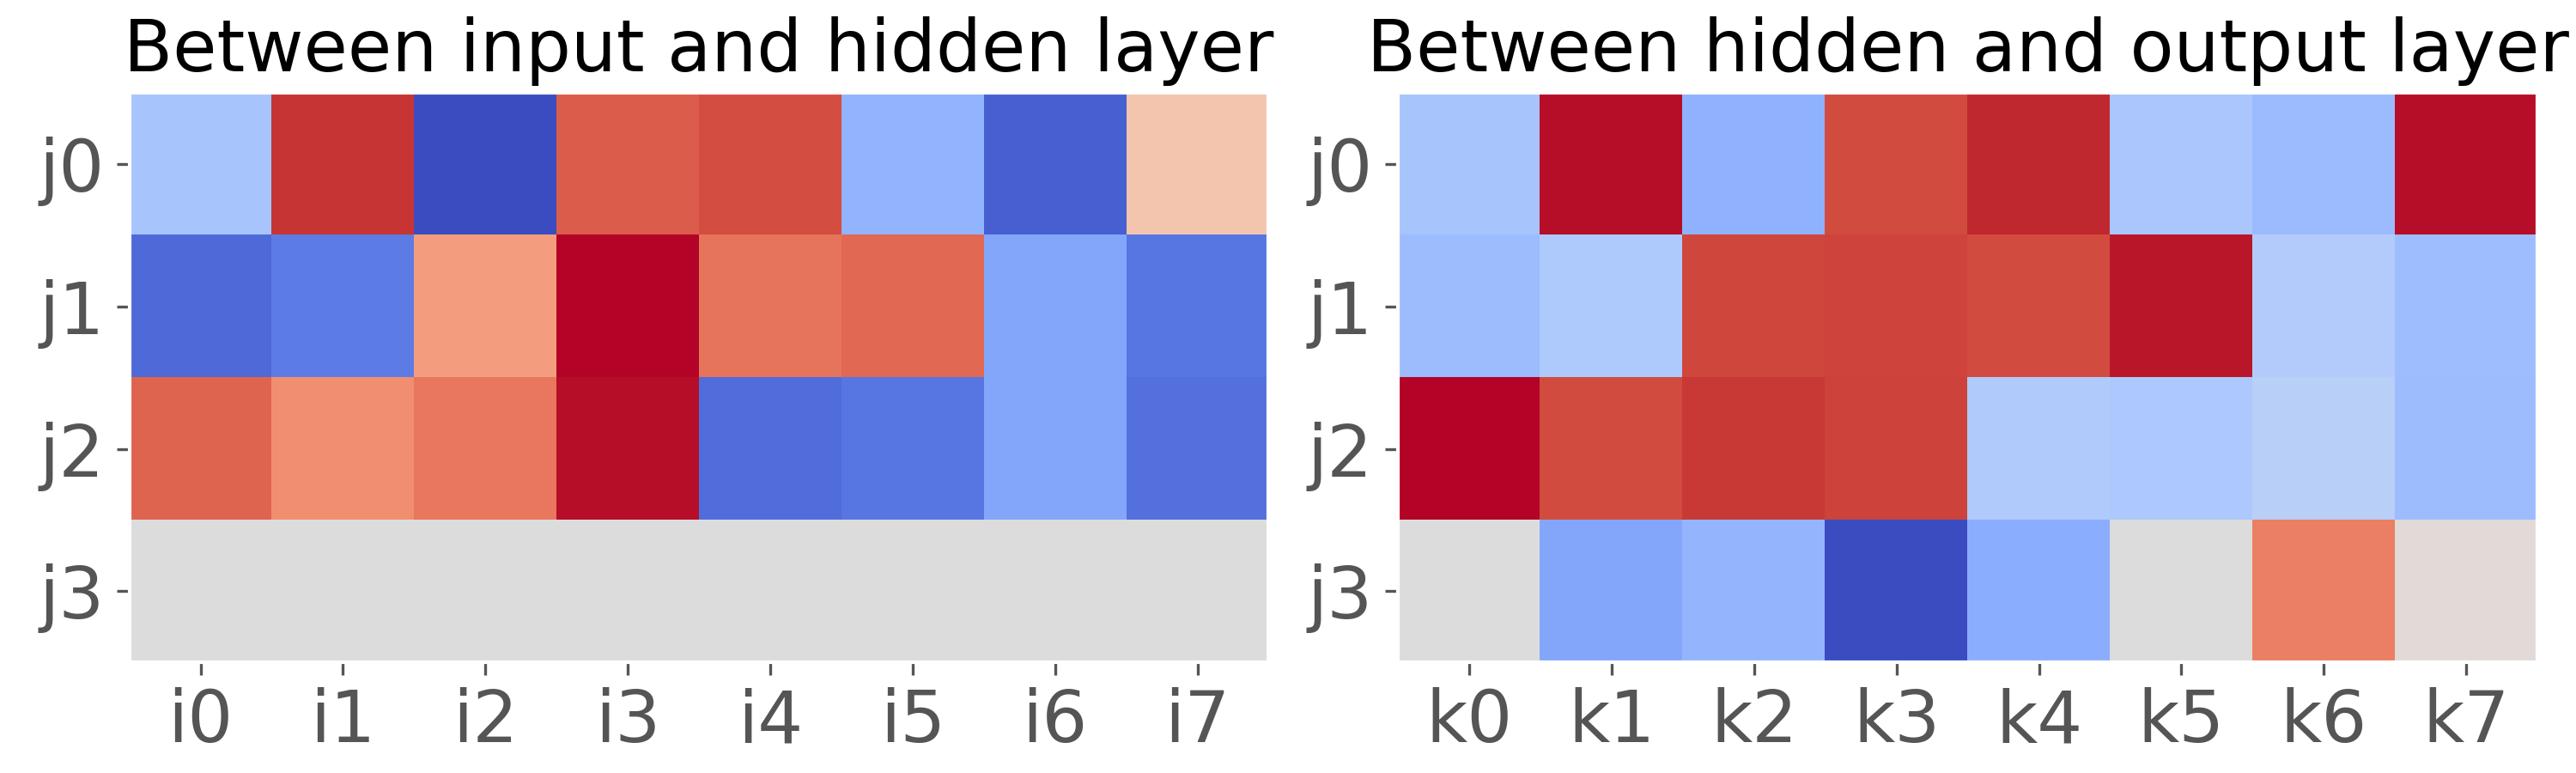
\includegraphics[width=10cm, height=3cm]{mlp_w}
    \caption{The network learns to mirror weights between the three layers}
    \label{fig:mlp_w}
\end{figure}

Without loss of generality, what the network has learned is to match the signs between mirrored pairs of weights ${W_{nj},\; W_{jn} \; \forall \; n \in [0,7], \; j \in [0,2]}$. For example, if $\mathbf{t}$ is \begin{pmatrix}1 & 0 & ... & 0\end{pmatrix}, then only $j_0$ and $k_0$ will fire, producing a large positive activation in $k_0$ because $W_{i0,j0}$ and $W_{j0,k0}$ have the same sign (does not matter whether positive or negative). The two other hidden units also have synergistic weights entering/leaving them, but they will stay silent because the inputs into those units is 0. 

\subsection{Encoding a 16-bit one-hot vector with 3 bits}

Is it possible to be even more efficient and encode a one-hot vector \textit{twice} the size as our previous vector, with 3 hidden units? If each hidden unit can represent 3 activation states, then we can encode up to a one-hot vector of length $3^n = 3^3 = 27$. Thus, this is theoretically possible. Of course, training will be slower, because there are more weights to adjust.

Here I train a multi-layer perceptron to encode with 3 untis a one-hot encoded vector of length \textbf{16}.

\begin{figure}[htbp]
    \centering
    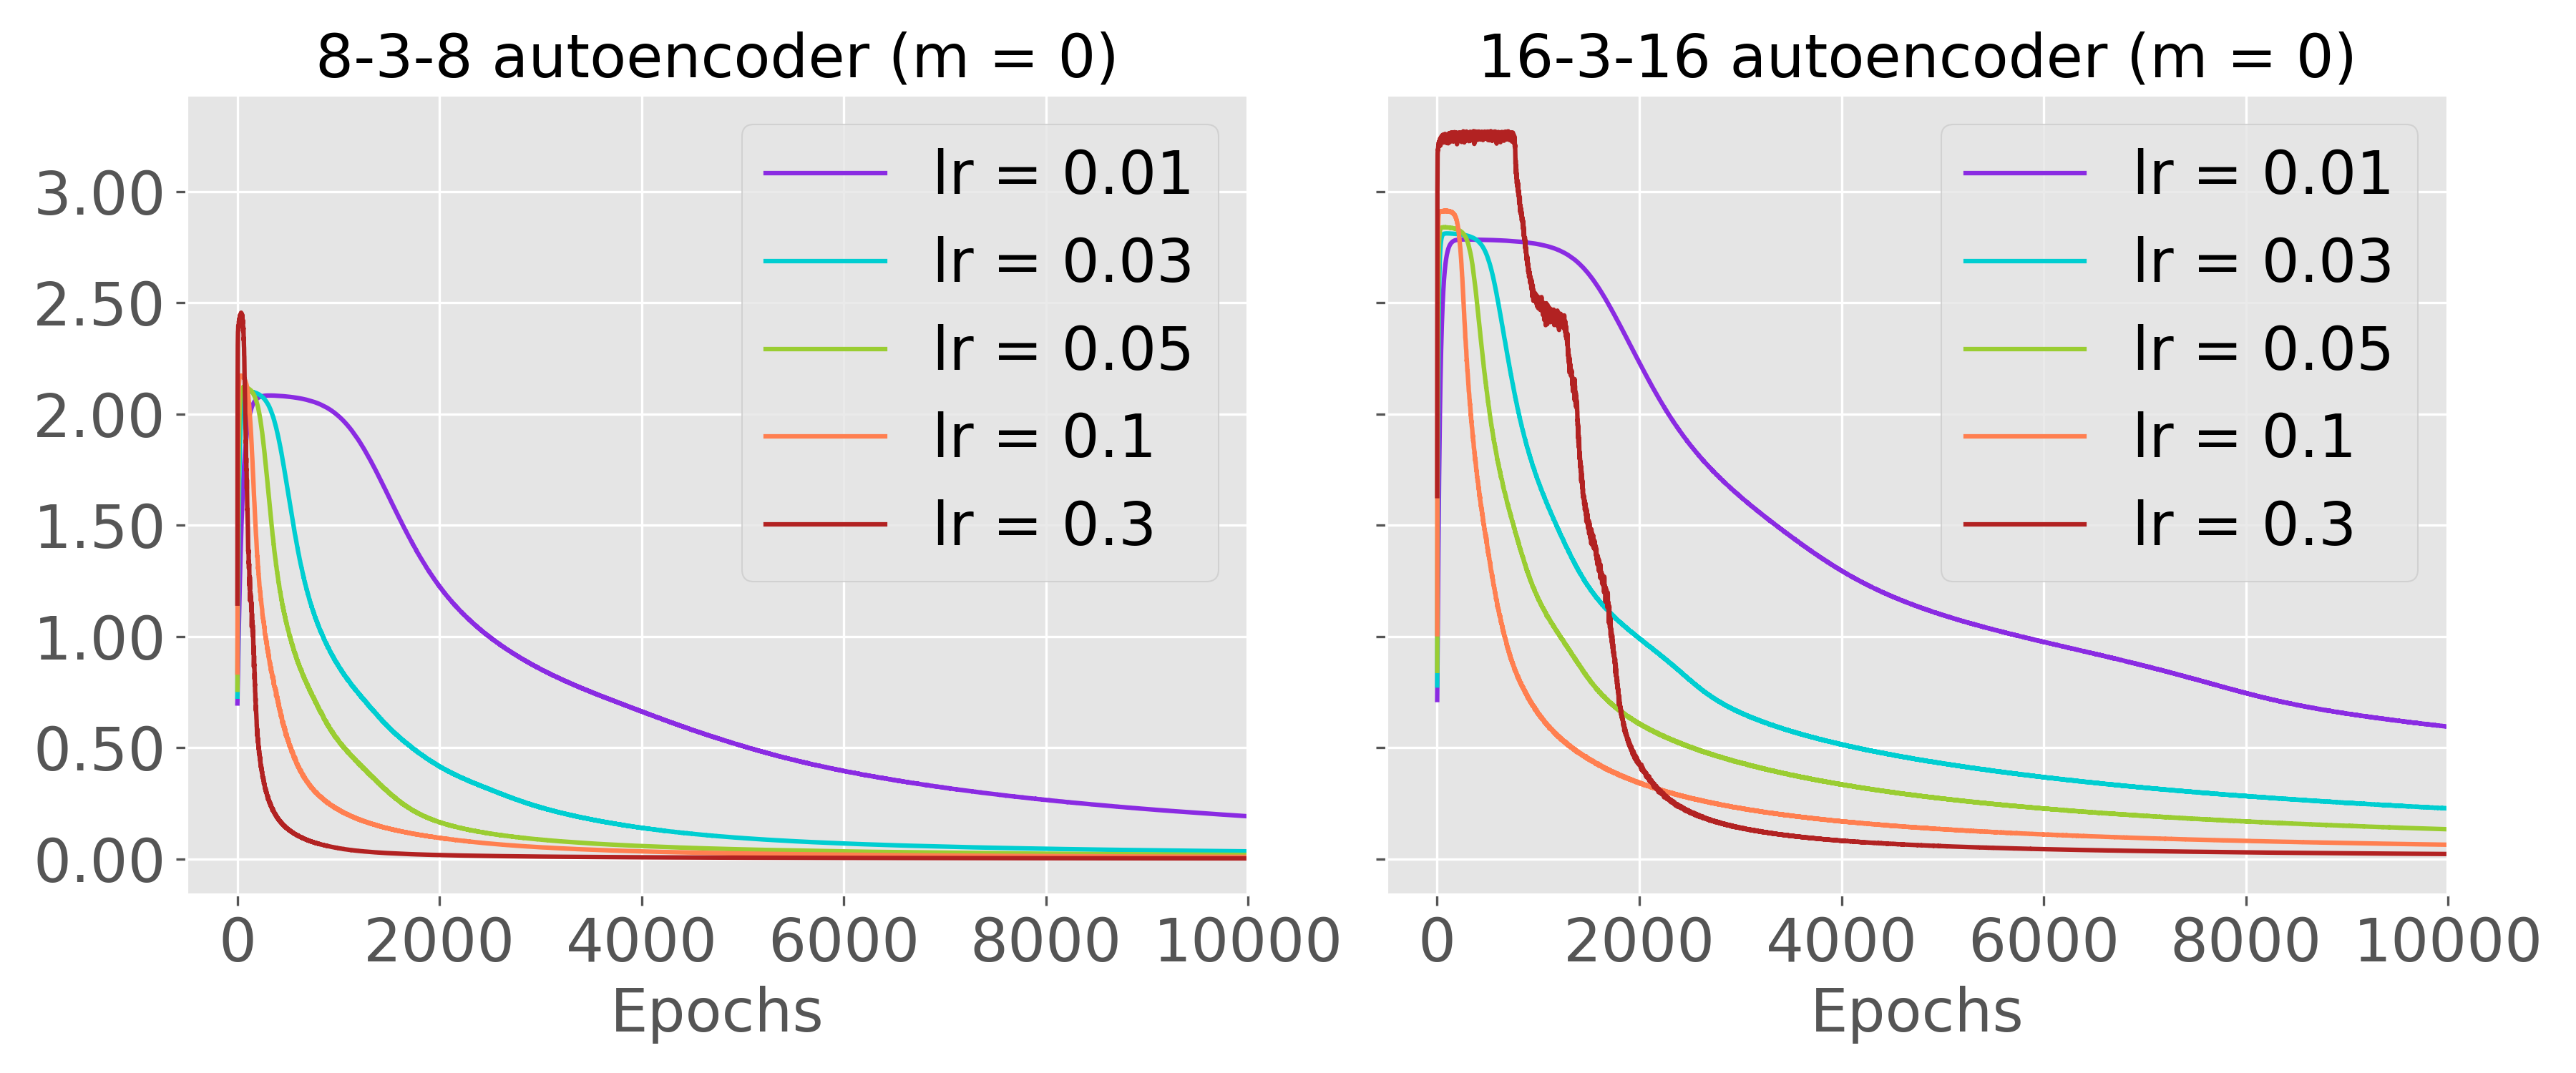
\includegraphics[width=12cm, height=5cm]{mlp_8_16}
    \caption{The 16-3-16 multi-layer perceptron trains slower across learning rates. Vertical axis is binary cross-entropy loss.}
    \label{fig:mlp_8_16}
\end{figure}


\begin{figure}
    \centering
    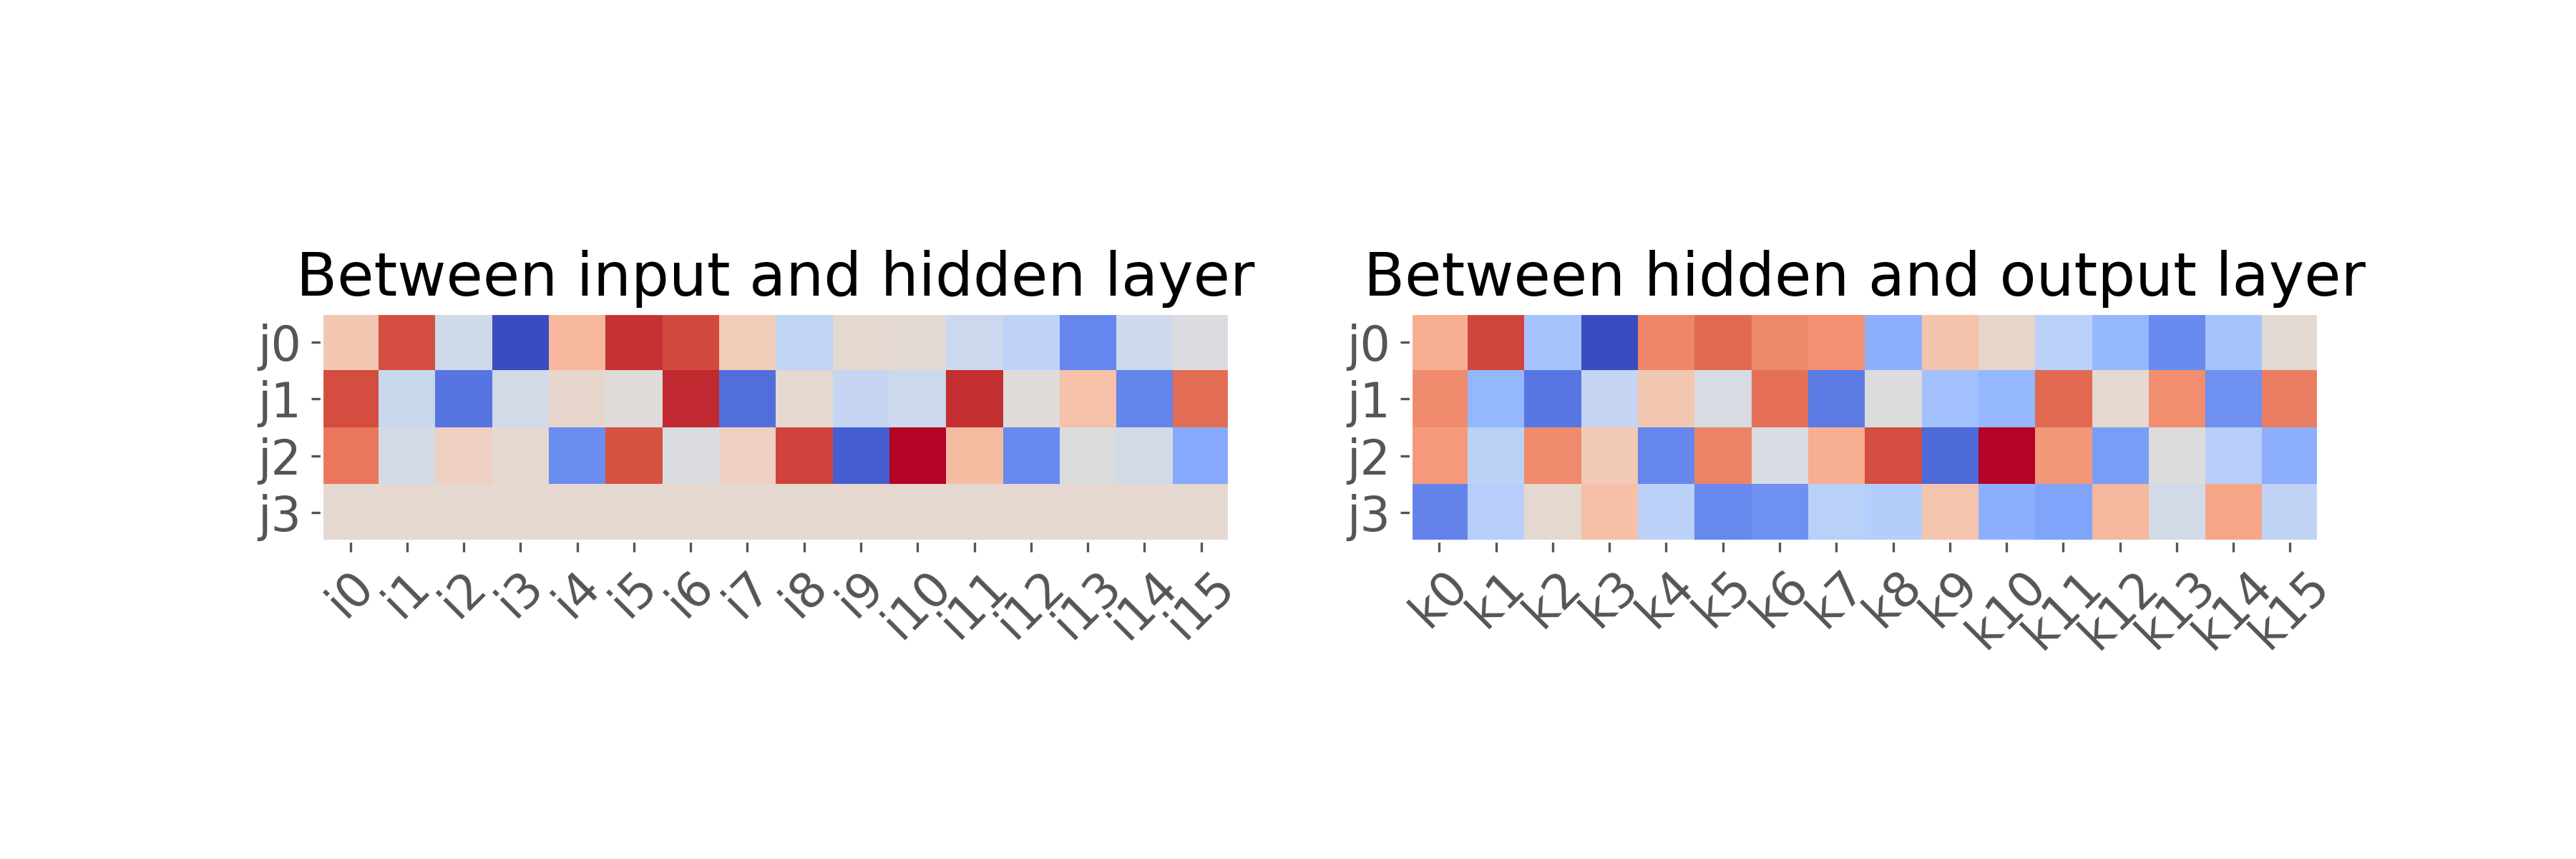
\includegraphics[height=3cm]{mlp16_w}
    \caption{Weights are again mirrored, and every hidden unit has 3 states - red, white and blue}
    \label{fig:mlp16_w}
\end{figure}



\end{document}